% !TeX root = ../main.tex

\chapter{基于特征增强的二值神经网络设计}

\section{概述}

虽然二值神经网络相比全精度浮点网络具有巨大的推理速度优势,但是其较弱的性能限制了二值神经网络的广泛应用。人们研究二值神经网络的目标是使其性能与浮点网络相当。为了提升二值神经网络网络的性能,必须像轻量化网络设计一样专门设计二值神经网络。High-Capacity Net\cite{expert}通过设计多个可选择的权重在ImageNet上达到了71.2\%的Top1准确率,但是该网络增加了较多的浮点计算量。

为了充分发掘二值神经网络的性能潜力,本文利用多二值特征图方法对二值特征进行增强,并结合二值友好网络结构设计,设计了全新的二值神经网络结构MFNet。其中多二值特征图方法提高了二值卷积的利用率,用更少的计算量实现更高的性能表现。二值友好网络结构设计针对二值网络进行了专门的设计,通过合理的排布模块中的网络层增强网络特征解析能力,并使用专用于二值网络的模块间激活函数以极低的浮点计算量为代价大幅提升二值网络的性能。

在上述方法的基础上,本文对网络结构进行了进一步优化。为了尽可能减少网络中的浮点计算量,本文对降采样和升维模块进行了专门的设计,将降采样和升维分别在两个二值卷积处实现。本文在残差连接上使用最大池化进行降采样,利用多二值特征图方法的通道扩增进行升维,从而避免了残差连接中浮点卷积的使用,极大的降低了网络的浮点计算量。二值网络使用浮点卷积作为首层卷积,本文对二值网络中的首层卷积进行研究,探究了首层卷积输出维数对二值网络的影响,通过尽可能减少首层卷积的输出维数进一步减少网络的浮点计算量。
本文对多二值特征图方法对网络通道数的需求进行了研究,通过合理的设置网络中的通道数高效地发挥多二值特征图方法的特征提取能力。

本章的主要贡献如下:

(1)本文将多二值特征图方法和二值友好结构设计相结合,设计了基于特征增强的二值神经网络MFNet。该网络充分利用了上述方法的优势,在ImageNet图像分类任务上取得了优异的性能表现。

(2)本文从降采样和升维模块、首层卷积等角度对MFNet网络进行设计,进一步降低了MFNet网络的浮点计算量,充分发挥了二值神经网络在推理速度上的优势。

\section{网络模块设计}

神经网络的主体结构是由网络模块堆叠而成的。本节介绍MFNet网络的基本模块和降采样与升维模块的设计方法。

\subsection{基本模块设计}

二值神经网络的设计目的是尽可能减少计算量,因此本文提出的MFNet参考了轻量化网络设计的思路。本文参考MobileNet\cite{mobilenet}的卷积设置,在一个网络模块中分别设置了一个$3 \times 3$卷积和一个$1 \times 1$卷积,但与MobileNet中使用的深度可分离卷积不同,MFNet中的所有卷积都是普通卷积。

MFNet的网络模块结构如图 \ref{fig:mfnet} 所示,为了实现多特征图方法的同时保持网络结构的简洁性,MFNet网络结构使用了多特征图方法的代替实现方法。MFNet在阈值为0的符号函数前插入特征扩增层,特征扩增层对一份浮点特征图施加不同的偏移量得到多张浮点特征图。多特征图方法中不同阈值的符号函数由不同偏移的浮点特征图和阈值为0的符号函数代替实现。根据前文的实验,考虑到计算量和精度的最佳权衡,MFNet网络的扩增倍数设置为2。

\begin{figure}[htb]
  \centering
  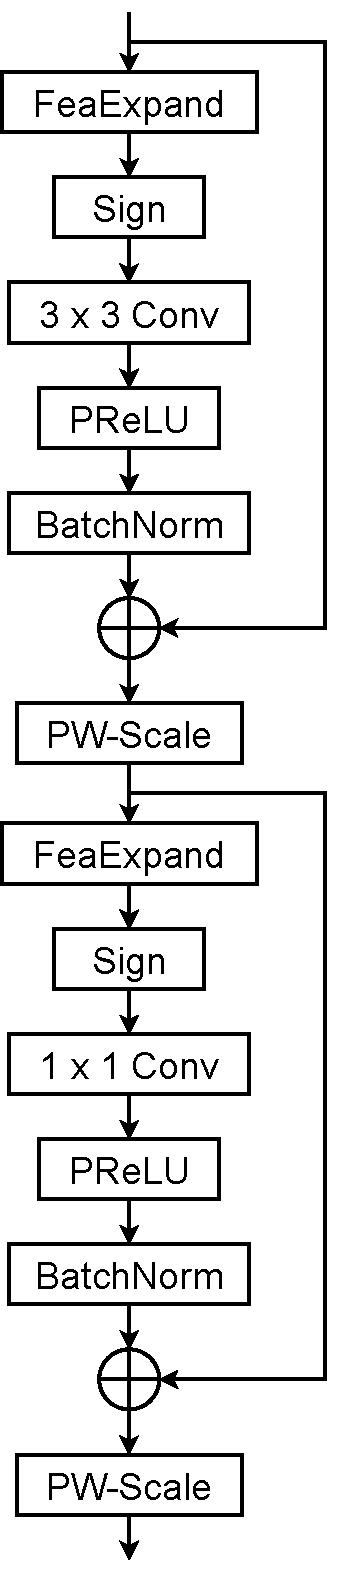
\includegraphics[width=0.22\textwidth]{mfnet.pdf}
  \caption{MFNet的网络模块结构示意图}
  \label{fig:mfnet}
\end{figure}

\subsection{降采样与升维模块设计}

目前的卷积神经网络一般采用金字塔结构,随着网络深度的增加,特征图的分辨率越来越小,通道数越来越多,一般卷积神经网络中会进行4次或5次的分辨率和通道数变化,每次将特征图的长和宽缩小为原来的一半,将通道数增加为原来的两倍。减小特征图的分辨率称为降采样操作,增加特征的通道数就是增加特征的维数,称为升维操作。分辨率和通道数相同且相邻的几个网络模块称为网络结构中的一个阶段。ResNet\cite{resnet}网络在每个阶段第一个模块中的第一个卷积处进行降采样和升维操作,其直接将该卷积替换为步长为2且输出通道数是输入通道数两倍的卷积。由于卷积输入与输出的的特征张量维数不同,该网络需要在残差连接上也加入一个$1 \times 1$卷积调整残差连接上特征图的分辨率和维数。

对于二值神经网络,如果将残差连接上的浮点卷积替换成二值卷积,网络的性能会明显下降。因此大多数二值网络在降采样和升维时的残差连接上直接使用了浮点$1 \times 1$卷积。这部分浮点卷积会带来较多的浮点计算量,为了减少此处浮点卷积带来的计算量,本文使用每个阶段第一个模块中的两个卷积分别进行降采样和升维操作。

降采样与升维模块如图 \ref{fig:mfnet_up} 所示,图中标注了每层特征图的通道数,该模块的输入通道数为$c$,输出通道数为$2c$。MFNet使用第一个卷积进行降采样,该卷积是步长为2,为了匹配主干和残差连接上特征图的分辨率,对残差连接上的特征图做步长为2的最大值池化操作。最大值池化几乎不增加网络的计算量,同时也能保证梯度在残差连接上的正常传递。MFNet使用第二个卷积进行升维,为了使主干和残差连接上特征图的通道数匹配,将残差连接的输入位置修改到特征扩增层下方。由于特征扩增倍数和升维使通道增加倍数均为2,此处的通道数刚好与主干通道数匹配。使用上述设计的降采样与升维方法,可以消除网络模块内的所有浮点卷积运算,大幅降低网络整体计算量。

\begin{figure}[htb]
  \centering
  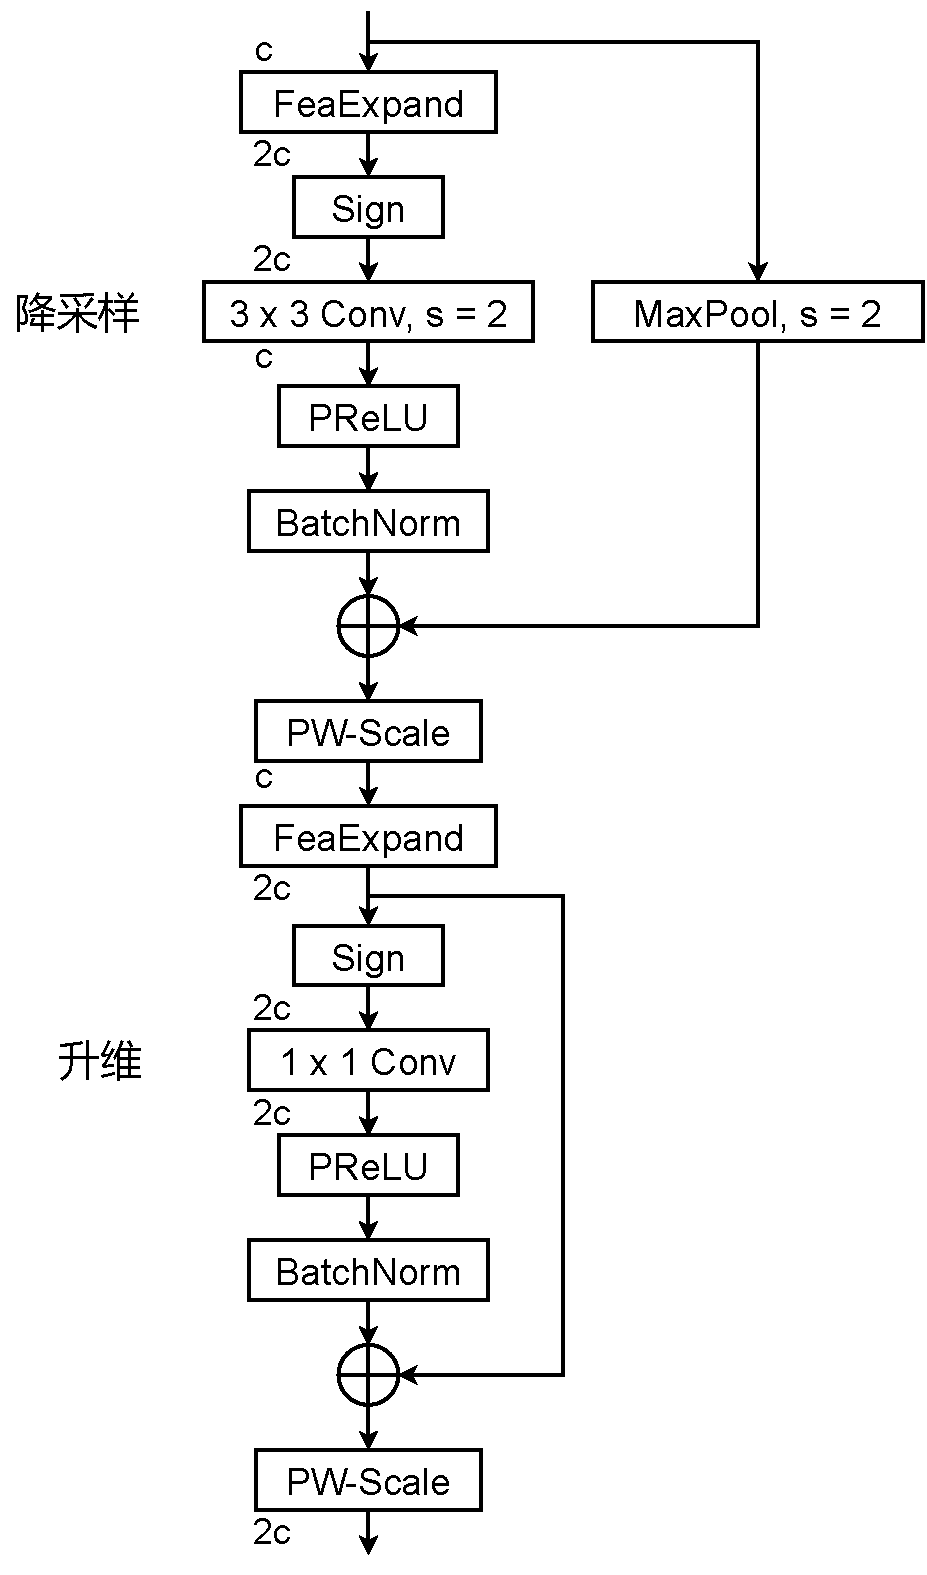
\includegraphics[width=0.6\textwidth]{mfnet_up.pdf}
  \caption{MFNet的降采样和升维模块结构示意图}
  \label{fig:mfnet_up}
\end{figure}

\section{整体网络结构设计}

在所有二值神经网络的设计中,都不对首层卷积和末层全连接层进行二值化,而是将它们保持浮点计算不变。神经网络的首层卷积用于从输入图像提取信息,由于首层卷积没有残差连接,将首层卷积二值化将会损失大量输入图像的信息,导致网络性能极差。神经网络的末层全连接层是图像分类器,将全连接层二值化将严重影响特征的分类能力,同样大幅削弱网络性能。本文的MFNet也采用相同的首层卷积和末层全连接的设置方法。当首层卷积的输出维数是64时,其计算量是末层全连接的约20倍。因此二值神经网络绝大部分浮点计算量源自首层卷积。

传统神经网络首层卷积的输出维数为64\cite{resnet},经过分析本文的MFNet使用32作为首层卷积的输出维数。得益于多二值特征图方法,从32维的浮点特征可以获得64维二值特征,所以MFNet第一个模块处理的特征维数仍然是64维。通过将首层卷积的输出维数减半,可以减少MFNet一半的浮点计算量。

本文的MFNet设计共分为五个阶段,每个阶段的输出分辨率和输出通道数如表 \ref{tab:41} 所示。其中阶段一只进行升维操作,不进行降采样操作,其他阶段都同时进行升维和降采样操作。阶段五结尾对每张特征图进行全局池化,得到1024维特征向量,然后经过全连接分类器得到类别评分。

MFNet的各阶段模块数如表 \ref{tab:41} 所示。传统神经网络多在分辨率$14 \times 14$,通道数为512的阶段堆叠最多的模块。为了与多二值特征方法相适应,本文的MFNet在分辨率$28 \times 28$,通道数为256的阶段堆叠最多的模块。这样做有两点原因,一是二值特征表示的信息极其有限,因此需要在更大的分辨率下进行最多次的特征提取。二是因为多二值特征图方法对特征的扩增作用,256通道的浮点特征可以相当于512通道的二值特征。

本文利用不同的模块数构建了不同计算量的MFNet网络,不同计算量网络的各阶段模块数如表 \ref{tab:41} 所示,其中MFNet-S是小型网络,MFNet-B是中型网络,MFNet-L是大型网络。每个网络的具体计算量参见表 \ref{tab:45}。

\begin{table}[h]
  \vspace{6pt}
  \centering
  \caption{MFNet系列网络各阶段模块数表}
  \label{tab:41}
  \begin{tabular}{cccccc}
    \toprule
    阶段名称 & 输出分辨率 & 输出通道数 & MFNet-S & MFNet-B & MFNet-L  \\
    \midrule
    主干  & $112\times112$ & 32 & - & - & - \\
    阶段一 & $112\times112$ & 64 & 2 & 2 & 2 \\
    阶段二 & $56\times56$ & 128  & 2 & 3 & 4 \\
    阶段三 & $28\times28$ & 256  & 3 & 7 & 8 \\
    阶段四 & $14\times14$ & 512  & 1 & 1 & 1 \\
    阶段五 & $7\times7$ & 1024   & 1 & 1 & 2  \\
    \bottomrule
  \end{tabular}
  \vspace{6pt}
\end{table}

\section{实验分析}

为了检验本文设计的MFNet网络的性能,本文使用ReActNet\cite{reactnet}网络的训练方法对MFNet系列网络进行训练,并与目前精度较高的其他二值神经网络的性能进行比较。

\subsection{实验细节}

本文使用ImageNet数据集训练和评估MFNet网络,为了公平比较,MFNet的训练策略与目前精度最高的二值网络ReActNet\cite{reactnet}相同。我们使用两阶段训练的方法训练MFNet,第一阶段只将激活值二值化,第二阶段载入第一阶段训练的权重,并将权重和激活值都二值化。我们使用Adam优化器进行训练,每个阶段各训练256个周期。训练的初始学习率设置为$5\text{e}^{-4}$,学习率使用线性下降策略,在训练结束时下降为0。第一阶段训练权重的衰减系数为$1\text{e}^{-5}$,模块中的PReLU函数和模块间的PW-Scale函数中的可学习参数均不进行权值衰减,第二阶段所有参数都不进行权值衰减。

本实验参考了ReActNet\cite{reactnet}的损失函数设置方法,在用于图像分类的交叉熵损失函数基础上添加了浮点网络蒸馏损失函数,蒸馏损失函数计算方法如公式 \eqref{eq:distill} 所示:

\begin{equation}
  \label{eq:distill}
  L_{distill} = -\frac{1}{n} \sum_{i = 1}^{n} \sum_{c} p_c^T(X_i)\log(\frac{p_c^S(X_i)}{p_c^T(X_i)})
\end{equation}
其中$n$表示训练集样本个数,$c$表示分类类别,$X_i$表示第$i$个样本的输入,$p_c^T(X_i)$和$p_c^S(X_i)$分别表示教师网络和学生网络计算得到的样本$X_i$是第$c$个类别的概率值。蒸馏损失函数计算了教师网络和学生网络预测的类别概率的KL散度。本文使用ResNet-34网络作为浮点教师网络,MFNet网络作为二值学生网络,总损失函数可以表示为:

\begin{equation}
  L = L_{ce} + L_{distill}
\end{equation}

MFNet网络的模块结构和固定阈值实验中的基准网络相似,本文使用手工搜索得到的-0.7和0.7作为多特征图方法的两个阈值取值。

\subsection{MFNet网络精度和计算量与其他二值网络比较}

本文设计的MFNet系列网络与其他用于图像分类的二值神经网络计算量和推理精度的比较如表 \ref{tab:45} 所示,除ResNet-18为浮点网络外,表中其他网络均为权重和激活值都二值化的二值网络。

\begin{table}[htb]
  \vspace{6pt}
  \centering
  \caption{MFNet与其他二值网络精度和计算量比较表}
  \label{tab:45}
  \begin{tabular}{cccccc}
    \toprule
    Architecture & \makecell{BOPs \\($\times10^9$)} & \makecell{FLOPs\\($\times10^8$)} & \makecell{OPs\\($\times10^8$)} & \makecell{Top1 \\ Acc(\%)} & \makecell{Top5 \\ Acc(\%)} \\
    \midrule
    ResNet-18 \cite{resnet} & 0 & 18.1 & 18.1 & 69.9 & 89.4 \\
    \hline
    XNOR-Net-18 \cite{xnornet} & 1.70 & 1.41 & 1.67 & 51.2 & 69.3 \\ 
    Bi-Real Net-18 \cite{birealnet} & 1.68 & 1.39 & 1.63 & 56.4 & 79.5 \\ 
    XNOE-Net++ \cite{xnornet++} & 1.70 & 1.41 & 1.67 & 57.1 & 79.9 \\ 
    PCNN \cite{pcnn} & - & - & 1.63 & 57.3 & 80.0 \\ 
    IR-Net \cite{irnet} & 1.68 & 1.30 & 1.57 & 58.1 & 80.0 \\ 
    CI-BCNN-18 \cite{cibcnn} & - & - & 1.63 & 59.9 & 84.2 \\ 
    Real-to-Bin \cite{realtobin} & 1.68 & 1.56 & 1.83 & 65.4 & 86.2 \\ 
    MeliusNetB \cite{meliusnet} & 5.72 & 1.06 & 1.96 & 65.7 & 85.9 \\ 
    ReActNet-A \cite{reactnet} & 4.82 & 0.12 & 0.87 & 69.4 & 88.6 \\ 
    High-Capacity Net \cite{expert} & 1.70 & 1.10 & 1.37 & 71.2 & 90.1 \\ 
    MFNet-S  & 1.81 & 0.12 & 0.40 & 65.5 & 86.0 \\
    MFNet-B  & 3.09 & 0.12 & 0.60 & 68.8 & 88.5 \\
    MFNet-L  & 4.63 & 0.12 & 0.84 & \textbf{71.5} & \textbf{90.1} \\
    \bottomrule
  \end{tabular}
  \vspace{6pt}
\end{table}

从表 \ref{tab:45} 中可以看到,在相似计算量的条件下,本文的MFNet-L取得了最高的71.5\%的ImageNet验证集精度。按照公式 \eqref{eq:ops} 的计算量换算标准,MFNet-L与浮点网络ResNet-18相比精度高了1.6\%,但计算量降低了20倍,充分验证了二值神经网络的加速效果。MFNet-L与部分二值网络的精度与计算量关系如图 \ref{fig:acc} 所示,图中更直观的展示了MFNet-L相比其他二值网络的优势。与ReActNet-A相比,MFNet-L在计算量几乎相同的条件下精度提高了2.1\%,这表明得益于多二值特征图方法,MFNet-L比ReActNet-A具有更强的二值特征提取能力,浮点特征二值化过程的信息损失更少。与High-Capacity Net相比,本文的MFNet-L具有更多的二值卷积计算,而High-Capacity Net则在网络模块中存在浮点卷积运算,在统一计算量标准下,MFNet-L以60\%的计算量取得了与High-Capacity Net几乎相同的精度,这表明本文的多二值特征图方法和二值友好网络结构更多的发掘了二值神经网络的潜力,更高效的利用了二值卷积的特征解析能力。

\begin{figure}[htb]
  \centering
  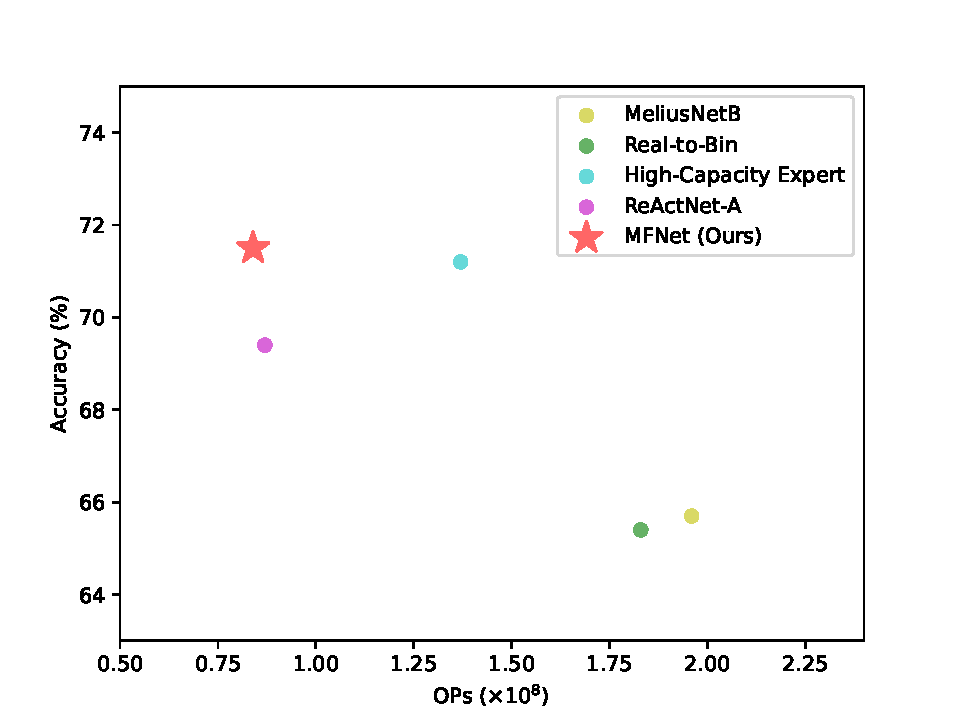
\includegraphics[width=0.8\textwidth]{fig1.pdf}
  \caption{MFNet与其他二值网络的精度与计算量关系图}
  \label{fig:acc}
\end{figure}

\section{本章小结}

在本章中,本文将多二值特征图方法和二值友好网络结构设计方法相结合,设计出全新的二值神经网络MFNet。本文从降采样与升维模块和网络整体通道数对MFNet进行设计,使MFNet具有尽可能少的浮点计算。实验表明本文提出的MFNet在ImageNet图像分类任务上超过了其他所有二值网络方法,在相同计算量下取得了最好的性能表现。